% === Begin Label Data ===
% ID: 301
% 难度星级: 
% 标签: 
% 备注: 数学建模
% 组卷引用次数: 0
% === End  Label Data ===

\begin{problem}{2008}{G}{江苏卷}{17}{函数}
17.（15 分）如图，某地有三家工厂，分别位于矩形 $ABCD$ 的两个顶点 $A$，$B$ 及 $CD$ 的中点 $P$ 处．$AB=20\,\text{km}$，$BC=10\,\text{km}$．为了处理这三家工厂的污水，现要在该矩形区域内（含边界）且与 $A$，$B$ 等距的一点 $O$ 处，建造一个污水处理厂，并铺设三条排污管道 $AO$，$BO$，$PO$．记铺设管道的总长度为 $y\,\text{km}$．

（1）按下列要求建立函数关系式：  
（Ⅰ）设 $\angle BAO=\theta$（$\text{rad}$），将 $y$ 表示成 $\theta$ 的函数；  
（Ⅱ）设 $OP=x$（$\text{km}$），将 $y$ 表示成 $x$ 的函数；  

（2）请你选用（1）中的一个函数关系确定污水处理厂的位置，使铺设的污水管道的总长度最短．
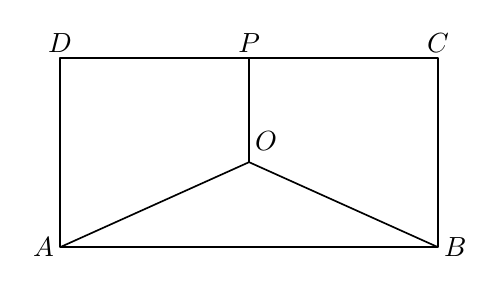
\begin{tikzpicture}[scale=1.2, line join=round]
    % 定义坐标 (按题意 AB=20, BC=10, 比例 2:1)
    \coordinate (A) at (0,0);
    \coordinate (B) at (4,0);
    \coordinate (C) at (4,2);
    \coordinate (D) at (0,2);
    \coordinate (P) at (2,2);
    % O点与A,B等距，故在AB的中垂线上，视觉上位置偏下
    \coordinate (O) at (2,0.9);

    % 绘制矩形边框
    \draw[semithick] (A) -- (B) -- (C) -- (D) -- cycle;
    
    % 绘制排污管道
    \draw[semithick] (A) -- (O) -- (B);
    \draw[semithick] (P) -- (O);

    % 标注字母
    \node[left, inner sep=2pt] at (A) {$A$};
    \node[right, inner sep=2pt] at (B) {$B$};
    \node[above, inner sep=2pt] at (C) {$C$};
    \node[above, inner sep=2pt] at (D) {$D$};
    \node[above, inner sep=2pt] at (P) {$P$};
    \node[above right, inner sep=2pt, yshift=2pt] at (O) {$O$};
\end{tikzpicture}
\end{problem}

\begin{answer}

\end{answer}

\begin{solutions}

\end{solutions}